\documentclass{article}
\usepackage[europeanresistors,americaninductors,americanvoltages,americancurrents,siunitx]{circuitikz}
\usepackage{pgfplots}
\usetikzlibrary{datavisualization}
\usetikzlibrary{datavisualization.formats.functions}
\usepgflibrary{arrows.meta}


\begin{document}
	
 	\begin{circuitikz} 
 		\draw (0,2) to[V_=$e(t)$] (0,0);
 		\draw (0,2) to[C=$C$] (4,2)	to[L=$L$] (4,0) to [R=$R$] (0,0);
 		\draw [->] (2,1.5) to [bend left=60,edge label'=$i(t)$] (2,0.5);
 	\end{circuitikz}

 	%\begin{circuitikz}[scale=1]
	\tikz{
		\draw (0,0) node[transformer core] (T) {}
		(T.A2) to ($(T.A2)+(-1,0)$) to [vC,l=$C$] ($(T.A2)+(-1,2)$)
		|- (T.A1);
		\draw [-{Circle[open]}](T.B2) to ($(T.B2)+(0.5,0)$);
		\draw [-{Circle[open]}](T.B1) to ($(T.B1)+(0.5,0)$);
	}
		%(T.B2) to[pDo] ($(T.B2)+(2,0)$) -| (3.5, -1)
		%(T.B1) to[pDo] ($(T.B1)+(2,0)$) -| (3.5, -1);
	%\end{circuitikz}		
 	
 	\begin{circuitikz}[scale=1]
		\ctikzset{bipoles/length=1cm} 
 		\draw	(0,2) to[V_=$e(t)$] (0,0);
 		\draw (0,2) to[C=$C$,v=$u_c$] (4,2) to[L=$L$] (4,0) to [R=$R$] (0,0);
 		\draw [->] (3,1.5) to [bend left=60,edge label'=$i(t)$] (3,0.5);
 	\end{circuitikz}

	\begin{circuitikz}[scale=1]
		\ctikzset{bipoles/length=0.8cm} 
 		\draw	(0,2) to[esource,l_=$e(t)$] (0,0);
 		\draw (0,2) to[C=$C$,v=$u_c$] (3,2) to [R=$R$] (3,0)--(0,0);
 		%\draw [->] (1.5,1.3) to [bend left=100,edge label'=$i(t)$] (1,0.3);
		\draw [->] (1.5,1.3) arc (90:-150:0.6 and 0.5);
		\draw (1.2,0.8) node[right] {$i(t)$} (0,0.6) node[left] {$-$}
		(0,1.4) node[left] {$+$};
 	\end{circuitikz}
 			
 	
 	\begin{circuitikz}
	 	\ctikzset{bipoles/length=1.4cm}
		\draw(0,0) to [L=1<\henry>](2.5,0) to [L=2<\henry>](5,0)
 			 		to	[R=1<\ohm>] (5,-2.5) to (5,-2.5)--(0,-2.5);
 		\draw	(0,0) to 	[R,l_=1<\ohm>] (0,-1.5) to [V_=$e(t)$](0,-2.5);
    	\draw	(2.5,0) to 	[C, l=1<\farad>,*-*] (2.5,-2.5)	;
    	\draw [->] (1.25,-0.5) to [bend left=65,edge label'=$i_1(t)$] (1.25,-2);
    	\draw [->] (3.5,-0.5) to [bend left=65,edge label=$i_2(t)$] (3.5,-2);
 	\end{circuitikz}
	\\~\\
 		 	

	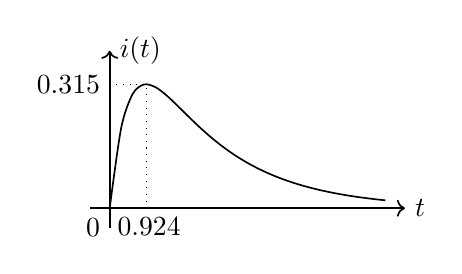
\begin{tikzpicture}[scale=0.5]
		\draw [semithick][->] (-0.5,0) -- (7.5,0) node[right] {$t$};
		\draw [semithick][->] (0,-0.5) -- (0,4) node[right] {$i(t)$} ;
		\draw (0,-0.5) node[left] {0} (0,3.15) node[left] {0.315}
			(1,0) node[below] {0.924};
		\draw [dotted] (0,3.15) -- (0.924,3.15) -- (0.924,0);
		 			
		\newcommand\SIGMA{6.66}
		%\datavisualization [school book axes, visualize as smooth line,x axis={label=$t$},y axis={label=$i(t)~A$}]
		\datavisualization [xy Cartesian, visualize as smooth line]
			data [format=function] {
			var x : interval [0:7];
		    func y = \SIGMA*(exp(-0.5*\value x)-exp(-2*\value x));};
	\end{tikzpicture}

	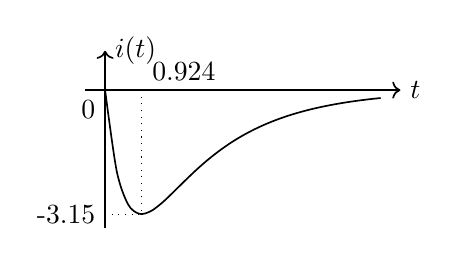
\begin{tikzpicture}[scale=0.5]
		\draw [semithick][->] (-0.5,0) -- (7.5,0) node[right] {$t$};
		\draw [semithick][->] (0,-3.5) -- (0,1) node[right] {$i(t)$} ;
		\draw (0,-0.5) node[left] {0} (0,-3.15) node[left] {-3.15}
						(2,0) node[above] {0.924};
		\draw [dotted] (0,-3.15) -- (0.924,-3.15) -- (0.924,0);
 		\newcommand\SIGMA{-6.66}
		%\datavisualization [school book axes, visualize as smooth line,x axis={label=$t$},y axis={label=$i(t)~A$}]
    	\datavisualization [xy Cartesian, visualize as smooth line]
			data [format=function] {
			var x : interval [0:7];
			func y = \SIGMA*(exp(-0.5*\value x)-exp(-2*\value x));};
	\end{tikzpicture}


  	
	\begin{circuitikz}[scale=1.4]
		\draw (0,0) to[C, l=10<\micro\farad>] (0,2) -- (0,3)
 		to[R, l=2.2<\kilo\ohm>] (4,3) -- (4,2)
 		to[L, l=12<\milli\henry>, i=$i_1$,v=b] (4,0) -- (0,0)
 		(4,2) { to[D*, *-*, color=red] (2,0) }
 		(0,2) to[R, l=1<\kilo\ohm>, *-] (2,2)
 		to[cV, i=1,v=$\SI{.3}{\kilo\ohm} i_1$] (4,2)
 		(2,0) to[I, i=1<\milli\ampere>, -*] (2,2) ;
	\end{circuitikz}
 
 	\begin{circuitikz}[scale=1.2]
	 	\draw(0,2) to[I=1<\milli\ampere>] (2,2)
		to[R, l_=2<\kilo\ohm>, *-*] (0,0)
		to[R, l_=2<\kilo\ohm>] (2,0)
		to[V, v_=2<\volt>] (2,2)
		to[spst, l=$t_0$] (4,2) -- (4,1.5)
		to [generic, i=$i_1$, v=$v_1$] (4,-.5) -- (4,-1.5)
		(0,2) -- (0,-1.5) to[V, v_=4<\volt>] (2,-1.5)
		to [R, l=1<\kilo\ohm>] (4,-1.5);

		\begin{scope}[xshift=6.5cm, yshift=.5cm]
 			\draw [->] (-2,0) -- (2.5,0) node[anchor=west] {$v_1/\SI{}\volt$};
 			\draw [->] (0,-2) -- (0,2) node[anchor=west] {$i_1/\SI{}{\milli\ampere}$} ;
 			\draw (-1,0) node[anchor=north] {-2} (1,0) node[anchor=south] {2}
 				(0,1) node[anchor=west] {4} (0,-1) node[anchor=east] {-4}
 				(2,0) node[anchor=north west] {4}
 				(-1.5,0) node[anchor=south east] {-3};
 			\draw [thick] (-2,-1) -- (-1,1) -- (1,-1) -- (2,0) -- (2.5,.5);
 			\draw [dotted] (-1,1) -- (-1,0) (1,-1) -- (1,0)
 				(-1,1) -- (0,1) (1,-1) -- (0,-1);
 		\end{scope}
 	\end{circuitikz}
\end{document}